\documentclass[11pt]{article}

\usepackage[margin=0.6in]{geometry}
\usepackage[T1]{fontenc}
\usepackage[utf8]{inputenc}
\usepackage{lmodern}
\usepackage{array}
\usepackage{booktabs}
\usepackage{graphicx}
\usepackage{float}
\usepackage{hyperref}
\usepackage{parskip}
\usepackage{ragged2e}
\usepackage{setspace}
\usepackage{needspace}
\usepackage[table]{xcolor}
\usepackage{tikz}
\usetikzlibrary{arrows.meta,positioning}
\usepackage[natbibapa]{apacite}

\definecolor{PrimaryRed}{HTML}{8B1E1E}
\definecolor{DeepNavy}{HTML}{15324A}
\definecolor{MidTeal}{HTML}{287D7A}
\definecolor{SoftBlue}{HTML}{DDEEFF}
\definecolor{SoftGreen}{HTML}{E4F1E8}
\definecolor{SoftGold}{HTML}{F8EDC7}
\definecolor{SoftRose}{HTML}{F5E2E7}
\definecolor{SoftGray}{HTML}{F4F4F4}

\hypersetup{
  colorlinks=true,
  linkcolor=DeepNavy,
  urlcolor=DeepNavy,
  citecolor=DeepNavy,
  pdftitle={Communication That Changes What Happens Next},
  pdfauthor={Piter Zacari Garcia Bautista},
  pdfsubject={EDE 448 Module 3 Journal},
  pdfkeywords={AAC, meaningful communication, access-to-agency, Puzzle Plan, EQUITAS}
}
\setlength{\parindent}{0pt}
\setstretch{1.08}
\bibliographystyle{apacite}
\newcommand{\reviewsection}[1]{%
  \par\Needspace{5\baselineskip}\addvspace{0.16in}%
  \noindent{\large\bfseries\color{PrimaryRed}#1}\par
  \vspace{0.05in}%
}

\begin{document}

\hypersetup{pageanchor=false}
\begin{titlepage}
\newgeometry{margin=0.6in}
\thispagestyle{empty}

\begin{center}
{\large University of Rochester\\}
{\normalsize Warner School of Education\\[0.15in]}

{\color{PrimaryRed}\rule{\textwidth}{1.4pt}}\\[0.12in]
{\Huge\bfseries Communication That Changes\\[0.07in]
What Happens Next}\\[0.15in]
{\huge Meaningful Communication, AAC,\\[0.07in]
and Evidence Justice}\\[0.18in]
{\Large EDE 448 --- Module 3 Journal}\\[0.12in]

\vfill

{\color{PrimaryRed}\rule{0.78\textwidth}{0.7pt}}\\[0.20in]

\colorbox{SoftBlue}{%
\parbox{0.88\textwidth}{%
\centering\small\vspace{0.02in}
\textbf{From Device Availability to Student Authorship}\\[0.05in]
Communication becomes meaningful when the learner has an accessible way to author varied messages and partners allow those messages to influence learning, relationships, support, and the environment.
}%
}
\end{center}

\vfill

\begin{center}
\renewcommand{\arraystretch}{1.18}
\setlength{\tabcolsep}{4pt}
\begin{tabular}{>{\bfseries\RaggedLeft\arraybackslash}p{1.65in} >{\RaggedRight\arraybackslash}p{5.0in}}
Student & Piter Zacari Garcia Bautista \\
Assignment & Module 3 Journal \\
Course & EDE 448 --- Communication and Positive Behavioral Supports for Students with Autism and Other Complex Needs \\
Essential Question & What does meaningful communication look like for students with complex needs? \\
Primary Sources & Norrie et al.; Downing et al.; Peckham-Hardin \\
Applied Evidence & Posted TD Snap review, Communication Support Plan, course portfolio, EDE448 Modules 1--2, K--5 teaching placement, and EDU486 Invisible Invaders camp \\
Interpretive Lenses & Puzzle Plan and EQUITAS \\
Due Date & August 10, 2026, 11:59 PM EDT \\
\end{tabular}
\end{center}

\vfill

\begin{center}
\begin{minipage}{0.92\textwidth}
\centering\itshape
A communication system is meaningful when the student can use it to challenge an interpretation, enter a relationship, and change what happens next.\\
{\color{PrimaryRed}\rule{4.5in}{0.8pt}}
\end{minipage}
\end{center}

\vfill

\begin{center}
\begin{minipage}{0.95\textwidth}
\small
This journal uses my Puzzle Plan, an interdisciplinary framework that connects lived experience, education, data, research, technology, and advocacy so that no single diagnosis, observation, behavior, or score is mistaken for the whole learner. EQUITAS is the equity-centered heart of that framework. It asks whose knowledge is included, what context is missing, how power and bias shape interpretation, and whether a decision expands dignity, agency, belonging, and access. Applied to Module 3, these commitments make communication support an evidence-and-justice problem: adults must examine not only whether a device or strategy is present, but whether the student gains authorship and influence.
\end{minipage}
\end{center}

\restoregeometry
\end{titlepage}
\hypersetup{pageanchor=true}
\pagenumbering{arabic}

\reviewsection{Meaningful Communication Is Authorship, Not Performance}

At the beginning of Module 3, I described assistive technology as a way to reduce barriers and AAC as a multimodal communication system rather than a single device. Gesture, gaze, objects, images, text, signs, low-tech boards, devices, and speech can all belong to that system. Communication access should not depend on age, a test score, diagnosis, or proving readiness. The module did not replace that understanding. It made the standard more demanding. My Module 1 journal, \textit{Who Gets to Name, Interpret, and Design?}, asked how labels, lived experience, and educational environments shape what the world recognizes as developmental difference \citep{garciabautista2026module1journal}. My Module 2 journal then asked who gains power after support. Module 3 joins those questions: who is recognized as the author of a message, which communication is treated as credible, and can that message alter the adult's interpretation or the environment?

Meaningful communication is not defined by speech, speed, eye contact, independent device use, or whether a response matches an adult's expectation. It exists when a student's message is recognized as theirs, understood or respectfully repaired, and able to influence learning, relationships, support, and what happens next. AAC can make that authorship more accessible, but device presence does not prove communication power. There is no age, cognitive score, or developmental milestone that a student must reach before communication support can help \citep{ashaAAC}. \citet{norrie2021context} make the difference between device presence and communication access visible. In their five-month study of one special-education school, only six of approximately 180 pupils with complex communication needs were active high-tech AAC users. Their findings locate barriers not only in a device or learner but in training, technical support, staffing, policy, infrastructure, and the fit between technology and daily life. The study changes the question from ``Why is the student not using the device?'' to ``What conditions make this communication system usable across real activities and partners?''

That distinction matters because a learner can technically possess AAC while having access to only a narrow adult agenda. A system limited to requesting food, answering teacher questions, or following directions does not provide the language needed to disagree, joke, ask an unexpected question, express identity, repair a misunderstanding, participate academically, or refuse. Meaningful communication must include functions that adults did not script in advance. \citet{downing2015classroom} move that responsibility into the general education classroom by asking educators to examine actual routines, exchanges, peer relationships, and communication opportunities. A student can be physically present and still have little access to authorship. Predictable routines may help a learner anticipate an exchange, but meaningful participation also requires vocabulary and partner support for unpredictable comments, questions, disagreement, humor, and repair. Communication cannot be reduced to selecting between two adult-approved choices.

\reviewsection{The Environment Determines Which Competence Becomes Visible}

This question is personal for me as a Latino Dominican, bilingual, neurodivergent, and chronically ill learner and educator. I know how quickly an access barrier can be rewritten as a character judgment. Fatigue can become lack of commitment. Processing time can become lack of knowledge. Language difference can become confusion. A quieter or delayed response can become lack of interest. Meaningful communication requires adults to examine the conditions under which competence is being judged. In my K--5 technology teaching placement, I saw participation change when I reduced language demands, modeled the exact technology steps, made the sequence visible, and allowed familiar tools to remain available. The learner's competence had not suddenly appeared; the conditions for showing it had changed. In one documented interaction, a Spanish-language interface did not stop progress because visual demonstration, pointing, and short directions carried the instruction while the student completed the task \citep{placementEvidence2026}. Language access and partner behavior were not extras around learning. They were part of the communication system.

My EDU486 Invisible Invaders camp work gives me another concrete picture of this principle. Youth could look, move, choose, handle tools, photograph, draw, write, explain, partner, pause, pass, or return. Identity Beads represented complementary contributions rather than ranking children by one performance. During evidence-to-action work and the showcase, youth could revise models, create advocacy messages, demonstrate, point, answer, ask, hold evidence, partner, or observe \citep{campEvidence2026}. Those routes were not all AAC, and I am not claiming that a particular camper used an AAC system. They do show how classroom design decides which forms of authorship become visible. A communication-rich classroom distributes ways to enter the work before a student is treated as disengaged, incapable, or unwilling.

\begin{figure}[!ht]
\centering
\newcommand{\agencybox}[2]{%
  \fcolorbox{PrimaryRed}{SoftBlue}{%
    \parbox[c][0.34in][c]{1.45in}{\centering\textbf{#1}\\[-0.01in]\small #2}%
  }%
}
\agencybox{Choose}{site, tool, and role}
\hspace{0.01in}{\color{PrimaryRed}$\longrightarrow$}\hspace{0.01in}
\agencybox{Contribute}{question, model, or message}
\hspace{0.01in}{\color{PrimaryRed}$\longrightarrow$}\hspace{0.01in}
\agencybox{Advocate}{vote, decline, or teach}
\hspace{0.01in}{\color{PrimaryRed}$\longrightarrow$}\hspace{0.01in}
\agencybox{Redesign}{time, access, and sequence}
\caption{Adapted from my Module 2, \textit{Who Has More Power After Support?} Invisible Invaders made agency observable through youth decisions and contributions, not by appearance, speech speed, or quiet compliance.}
\label{fig:camp-agency}
\end{figure}

My Module 3 paper, \textit{Communication That Travels With the Student: A Neurodiversity-Affirming, Culturally and Health Responsive Support Plan}, turned those lessons into a prospective plan for three fictional composite students \citep{garciabautista2026communicationplan}. Mateo made bilingual and culturally sustaining access visible; Eli made speech and multimodal access visible; and Luca made chronic illness, body state, privacy, low speech, and speech-related trauma visible. Their profiles are fictional, while the support strategies are grounded in de-identified camp and placement evidence. Together, the profiles kept me from designing for an abstract ``AAC student.'' A dependable system must survive changes in language, energy, pain, partner, tool, setting, routine, and willingness to speak.

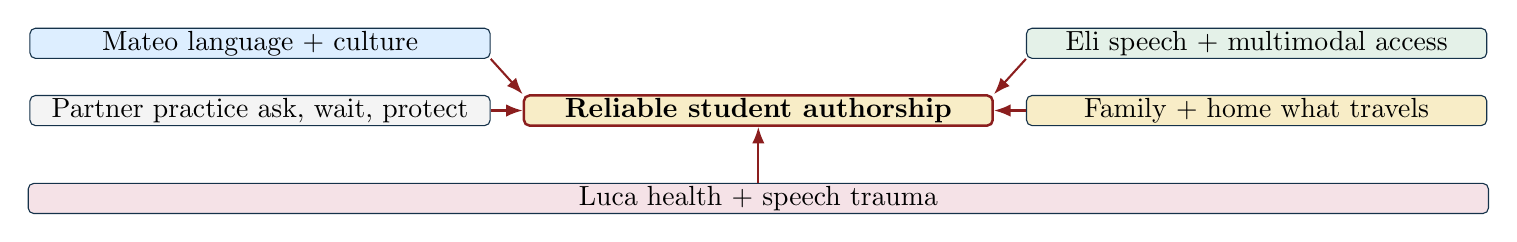
\begin{tikzpicture}[
  piece/.style={
    draw=DeepNavy,
    rounded corners=2pt,
    text width=4.10in,
    align=center,
    font=\normalsize,
    inner xsep=-65pt,
    inner ysep=1pt
  },
  topwide/.style={
    draw=DeepNavy,
    rounded corners=2pt,
    text width=4.10in,
    align=center,
    font=\normalsize,
    inner xsep=-65pt,
    inner ysep=1pt
  },
  bottomwide/.style={
    draw=DeepNavy,
    rounded corners=2pt,
    text width=9.10in,
    align=center,
    font=\normalsize,
    inner xsep=-65pt,
    inner ysep=1pt
  },
  centerpiece/.style={
    draw=PrimaryRed,
    line width=0.9pt,
    rounded corners=2pt,
    fill=SoftGold,
    text width=2.15in,
    align=center,
    font=\normalsize\bfseries,
    inner xsep=7pt,
    inner ysep=1pt
  },
  flow/.style={
    -{Latex[length=2.1mm]},
    line width=0.75pt,
    draw=PrimaryRed
  }
]

% Center
\node[centerpiece] (center)
  {Reliable student authorship};

% Middle left/right
\node[piece, fill=SoftGray,
  left=0.16in of center]
  (partner) {Partner practice ask, wait, protect};

\node[piece, fill=SoftGold,
  right=0.16in of center]
  (family) {Family + home what travels};

% Full-width top left/right
\node[topwide, fill=SoftBlue,
  above=0.18in of partner]
  (mateo) {Mateo language + culture};

\node[topwide, fill=SoftGreen,
  above=0.18in of family]
  (eli) {Eli speech + multimodal access};

% Full combined-width bottom
\node[bottomwide, fill=SoftRose,
  below=0.28in of center]
  (luca) {Luca health + speech trauma};

% Connections
\draw[flow] (mateo.south east) -- (center.north west);
\draw[flow] (eli.south west) -- (center.north east);
\draw[flow] (partner.east) -- (center.west);
\draw[flow] (family.west) -- (center.east);
\draw[flow] (luca.north) -- (center.south);

\end{tikzpicture}

\Needspace{5\baselineskip}
That plan also forced adult behavior into the intervention. Premature suggestions can replace a student's idea; taking over work can erase authorship; rigid pacing can make fatigue look like a learner deficit; and visible adult dysregulation can make communication unsafe. Partner training must therefore include asking before helping, keeping hands off student work without permission, waiting, noticing all reliable modes, returning control after assistance, and repairing when adult behavior restricts access.

\reviewsection{Communication, Behavior, and the Reliability of Adult Response}

\citet{peckhamhardin2015behavior} add another important dimension: actions that adults label challenging may be connected to a message that does not yet have a reliable pathway. Functional communication support begins by investigating the purpose, teaching an accessible alternative, and ensuring that partners honor the message. A break message that never produces a break teaches the learner that the new route is less reliable than the action adults are trying to replace. This builds on my submitted paper, \textit{From Compliance to Communication: Prevent--Teach--Reinforce Planning Through Access, Agency, and Richer Evidence}, without recreating its behavior plan \citep{garciabautista2026ptr}. That paper examined how allowing a familiar laptop to coexist with hands-on materials removed an unnecessary either-or condition. Module 3 adds the language and partner question: how could the learner say, ``keep this,'' ``different order,'' ``show me,'' ``not yet,'' or ``I meant something else'' before an adult completes the interpretation?

My posted \textit{AAC Review: TD Snap} made the implementation test concrete \citep{garciabautista2026tdsnap}. TD Snap offers multiple page sets, access routes, editing tools, bilingual Motor Plan options, and printable low-tech materials. Its value is not the number of features. Its value depends on feature matching, personalized vocabulary, backup access, partner practice, and whether the communicator can do more than request. In the fictional plan, Mateo would need Spanish--English vocabulary and family language; Eli would need robust multimodal access; and Luca would need easy access to health, privacy, fatigue, pacing, and repair messages. A classmate's review of the same tool added a useful EQUITAS question by placing customizable photographs beside the recurring subscription cost. Personal photographs can connect AAC to familiar people, activities, and interests; for a culturally and linguistically diverse student, personalization should also protect names, home-language vocabulary, family relationships, humor, and identity. Yet a feature is not accessible if a school can introduce it and the student or family cannot sustain it across home, summer, transitions, or a funding change. The team must decide who will pay, maintain an effective low-tech backup, and ask whether the student's voice remains available when the app or speech output is not.

\begin{figure}[!ht]
\centering
\newcommand{\commbox}[2]{%
  \fcolorbox{PrimaryRed}{SoftBlue}{%
    \parbox[c][0.68in][c]{1.45in}{\centering\textbf{#1}\\[-0.02in]\small #2}%
  }%
}
\commbox{Student Meaning}{comment, question, refusal, repair}
\hspace{0.01in}{\color{PrimaryRed}$\longrightarrow$}\hspace{0.01in}
\commbox{Access Route}{touch, gaze, gesture, symbol, text}
\hspace{0.01in}{\color{PrimaryRed}$\longrightarrow$}\hspace{0.01in}
\commbox{Partner Practice}{model, wait, notice, confirm, act}
\hspace{0.01in}{\color{PrimaryRed}$\longrightarrow$}\hspace{0.01in}
\commbox{Agency}{message changes what happens next}
\caption{My Module 3 access-to-agency synthesis. A device is one route inside a communication system; authorship depends on matched access and a partner response that lets the message matter.}
\label{fig:access-to-agency}
\end{figure}

\reviewsection{Puzzle Plan, EQUITAS, and Evidence Justice}

The Puzzle Plan is my interdisciplinary framework for bringing lived experience, education, data, research, technology, and advocacy together so that no diagnosis, observation, behavior, or score stands alone. EQUITAS is the equity-centered heart of that framework. It asks whose knowledge is included, what context is missing, how power and bias shape interpretation, and whether a support increases dignity, agency, belonging, and access. Through the Puzzle Plan and EQUITAS, communication support becomes evidence justice. When accessible modes are missing, schools can mistake speech, speed, or compliance for competence. A fair record would document the student's message, available modes, environmental conditions, partner response, breakdowns, successful repairs, family knowledge, and response to support. Even a home--school log can either increase or restrict power. A list of warnings, sitting, following directions, and good/fair/poor ratings tells adults about adult expectations. A student-centered record asks what the learner communicated, what worked, what barrier should change, and what the student wants shared.

\reviewsection{Media: Access Changes Who Can Enter the Public Record}

In the Module 3 documentary \textit{Wretches and Jabberers}, Tracy Thresher and Larry Bissonnette are autistic adults with limited speech who had been presumed intellectually incapable and excluded from ordinary schooling. After gaining access to typing, they traveled internationally to challenge public assumptions about disability and intelligence \citep{wurzburg2013wretches}. The meaningful change is not that adults gave them competence. An accessible route made their existing authorship harder to dismiss and allowed their messages to change the public conversation. This connects to \citet{norrie2021context}: a device alone does not create agency. The route must remain usable, partners must treat the message as consequential, and support must preserve authorship. In my classroom, I must neither presume incompetence because speech is limited nor treat one method as universal proof. I must provide multiple routes, confirm meaning respectfully, and let student messages revise instruction and support.

\reviewsection{What I Will Carry Into My Classroom}

In my future classroom, I will treat AAC as a continuously revised multimodal system rather than one device. Students need vocabulary for choosing, refusing, commenting, asking, joking, participating academically, expressing sensory and health needs, protecting privacy, and repairing misunderstandings. They need primary and backup options that travel through arrival, instruction, transitions, group work, lunch, dismissal, home, illness, absence, and re-entry. Adults and peers need to model, wait, notice, confirm, and act without requiring performance or taking over the student's voice. The team must also notice when a gesture, facial expression, object, written message, or pause already communicates effectively rather than demanding device repetition to make the message look more conventional \citep{mirenda2015aids}.

My central measure remains the one established in my Module 2 journal, \textit{Who Has More Power After Support?} \citep{garciabautista2026module2journal}. After communication support is introduced, can the student author more messages, enter more relationships, challenge an interpretation, protect a boundary, and influence what happens next? If support reduces visible behavior while adult control remains untouched, communication is still being managed rather than respected. Meaningful communication therefore looks like more than access to words. It looks like a learner being recognized as the author of a message that matters. It looks like partners who can tolerate being corrected and plans that change when the communicator shows that a support is not working. It looks like family knowledge traveling into school and student-authored information traveling home. Most of all, it looks like a student having something important to say, an accessible way to say it, and enough power for the message to change the world around them.


\clearpage
\footnotesize
\bibliography{references}

\end{document}
